\documentclass[a4paper,12pt]{article}
\usepackage{amsmath}
\usepackage{graphicx}
\usepackage{tikz}
\usepackage[margin=1in]{geometry}
\usepackage{caption}
\usepackage{authblk}
\usepackage{multirow}
\usepackage{graphicx}
\usepackage{amsmath}
\usepackage{amsmath}
\usepackage{graphicx}
\usepackage{tikz}
\usepackage[margin=1in]{geometry}
\usepackage{caption}
\usepackage{authblk}
\usepackage{multirow}
\usepackage{amsmath}
\usepackage{xcolor}
\usepackage{biblatex}
\usepackage{rotating}
\usepackage{multicol}
\usepackage{float}
\usepackage{enumitem}
\usepackage{subcaption}
\usepackage{hyperref}
\usepackage[table]{xcolor}
\hypersetup{
    colorlinks=true,
    linkcolor=blue,
    }
\usetikzlibrary{positioning, shapes, arrows.meta, calc}
\usepackage[label=corner]{karnaugh-map}


\geometry{top=1in, bottom=1in, left=1in, right=1in}

\begin{document}

\begin{center}
    \textbf{CSE 210} \\
    \textbf{Computer Architecture Sessional} \\[.8cm]
    \textbf{Assignment-2: 32-bit Floating Point Adder Simulation} \\[1cm]
    \textbf{Section -- C2} \\
    \textbf{Group -- 07} \\[5cm]
\end{center}

\noindent\textbf{Members of the Group:}
\begin{enumerate}
    \item 2105151 -- Md.Sani Alam Khan Piyes
    \item 2105152 -- Sudip Kumar Saha
    \item 2105167 -- Samyo Pramanik
    \item 2105172 -- Mezba-Us-Saleheen
\end{enumerate}
\newpage

\section{Introduction}

A computer representation of a real number with a fixed number of digits before
and after the decimal point (or radix point in a more general sense) is called
a floating point number. A floating point adder is a digital circuit that works
with floating point numbers to add and subtract. Numbers that are too large or
too small to be accurately represented by integer representations can be
represented using this method.

Three fields make up the floating point representation of a number: the sign
bit, the exponent field, and the mantissa field. The sign bit represents the
sign, either positive or negative. To express a wide range of values, the
exponent field permits the significand to be multiplied by a power of the base
using a fixed amount of bits in a biased form. The bias needs to be deducted
from the stored bits in order to get the real exponent. The fractional portion
of the number, or mantissa, is made up of the digits that come after the
decimal point. The sign bit, exponent field, and mantissa in this
implementation use 1, 9, and 22 bits, respectively. Thus, the exponent bias for
our problem would be $2^{9 - 1} - 1 = 255$.

In order to add two numbers, a floating point adder first aligns their decimal
points before adding their mantissas. After necessary shifts and related
modifications (increment/decrement), the result’s exponent is fixed.
Normalization and rounding are performed afterwards. The signs of the two
integers being added determine the sign of the outcome.

Applications for floating point adders include financial modeling, computer
graphics, and calculations in science and engineering. Because co-processors
can be computationally demanding, it is utilized in them to do quick,
hardware-accelerated floating point arithmetic. These calculations can be
completed far more quickly by a specialized floating point adder than by the
main processor. Applications requiring high-precision floating point
calculations, such as data analysis and scientific simulations, may find this
to be especially crucial.

\subsection{Floating Point Representation}

According to IEEE 754 standard, a floating-point number is delineated by a trio
of elements: a sign bit, an exponent, and a fraction (alternatively termed
mantissa or significand). The general structure adheres to the formula:

\[
    (-1)^{\text{sign}} \times (1 + \text{fraction}) \times 2^{\text{exponent} - \text{bias}}
\]
In our assignment,we have exponents of 9 bits and mantissa of 22 bits.

\begin{table}[h]
    \centering
    \begin{tabular}{|c|c|}
        \hline
        Bit Number & Portion           \\
        \hline
        31         & Sign (S)          \\
        30--22     & Exponent          \\
        21--0      & Fraction/Mantissa \\
        \hline
    \end{tabular}
    \caption{Bit Ranges of Floating-Point Number}
    \label{tab:floating_point_bits}
\end{table}

Each component holds specific significance:

\begin{itemize}
    \item Sign bit: Denoting the sign of the number, with 0 for positive and 1 for
          negative.
    \item Exponent: Denoting the exponent of 2 by which the fraction undergoes
          multiplication.
    \item Fraction: Representing the actual fractional segment of the number, often
          normalized to commence with a leading 1.

\end{itemize}

The normalized significand, residing in the range \(1.0 \leq \lvert
\text{significand} \rvert < 2.0\), consistently incorporates a leading
pre-binary-point 1 bit. This obviates the need for explicit representation,
commonly denoted as the hidden bit. The normalized significand is essentially
synonymous with the fraction, featuring the restored "1." at its forefront.

The bias, a constant, is incorporated to facilitate the representation of the
exponent using a signed integer, thereby accommodating both positive and
negative exponents.Here the bias is 255.

\subsection{Range }

\begin{itemize}
    \item Extremely small numbers, in proximity to zero, manifest with a diminished
          exponent and a fraction featuring leading zeros.
    \item Extremely large numbers are portrayed with an elevated exponent.
\end{itemize}

In a floating-point adder with a 22-bit mantissa and an 9-bit exponent, the
largest and smallest representable positive normalized numbers are determined
by the range of exponents and the precision of the mantissa.

For the largest positive number, the exponent is set to its maximum value of
255, and the mantissa is the maximum value for a 22-bit representation. The
binary representation is \(1.11111111111111111111 \times 2^{255}\). In
approximate decimal form, this represents a number of approximately
\(3.402823466 \times 10^{76}\).

For the smallest positive normalized number, the exponent is set to its minimum
value of -254, and the mantissa is the minimum value (just the implicit leading
bit). The binary representation is \(1.00000000000000000000 \times 2^{-254}\),
approximately equal to \(5.562684646268003 \times 10^{-77}\) in decimal.

These values encapsulate the range of positive normalized numbers that can be
precisely represented by your floating-point adder with a 22-bit mantissa and
an 9-bit exponent. It's crucial to note that these approximations are subject
to the inherent limitations of representing real numbers in a finite binary
format.

\subsection{EEE 754 encoding of floating point numbers}
\begin{table}[h]
    \centering
    \begin{tabular}{|c|c|c|}
        \hline
        Exponent & Fraction & Object Represented          \\
        \hline
        0        & 0        & 0                           \\
        \hline
        0        & Non Zero & $\pm$ Denormalized Number   \\
        \hline
        1--510   & Anything & $\pm$ Floating Point Number \\
        \hline
        511      & 0        & $\pm$ Infinity              \\
        \hline
        511      & Nonzero  & NaN (Not a Number)          \\
        \hline
    \end{tabular}
    \caption{EEE 754 Encoding}
    \label{EEE 754 Encoding}
\end{table}

\subsection{Denormalized Number}
The denormalized numbers in IEEE 754 floating-point representation are a
special category of values that are smaller than normal numbers. They are used
to allow for gradual underflow, where numbers get extremely close to zero with
diminishing precision. Denormalized numbers have an exponent of all zeros and a
hidden bit set to zero. The formula for denormalized numbers is:

\[ \text{Denormalized Number} = (-1)^{\text{sign}} \times (0 + \text{Fraction}) \times 2^{-\text{exponent}_{\text{min}}} \]

Where: -- \(\text{sign}\) is the sign bit (either 0 or 1), --
\(\text{Fraction}\) is the fractional part of the number (including the hidden
bit, which is 0 for denormalized numbers), -- \(\text{exponent}_{\text{min}}\)
is the minimum representable exponent value.

Denormalized numbers have a smaller exponent range compared to normalized
numbers, and they allow for a smooth transition to zero, ensuring that
precision degrades gradually as the numbers get smaller.

For example, in single-precision format, the smallest denormalized number is
represented as:

\[ 0.\underbrace{0000 0000 0000 0000 0000 01}_{\text{Fraction}} \times 2^{-254} \]

Which is equivalent to \(1.0 \times 2^{-276}\). This is considerably smaller
than the smallest positive normalized number, which is \(1.0000 0000 0000 0000
0000 00 \times 2^{-254}\). Denormalized numbers play a crucial role in
maintaining precision for very small values close to zero in floating-point
arithmetic.

\subsection{Floating Point Number Addition}

Performing floating-point addition involves several steps:

\textbf{Example:}
Consider two normalized numbers in IEEE 754 single-precision format:
\[
    A = (-1)^0 \times 1.011 \times 2^3 \quad \text{and} \quad B = (-1)^1 \times 1.101 \times 2^2
\]

\textbf{Step 1: Aligning Exponents}
Let us Identify the number with the smaller exponent and adjust its mantissa and exponent to match the larger one. Since \( B \) has a smaller exponent, we need to align it with \( A \). We shift the mantissa of \( B \) to the right and decrease its exponent by 1:
\[
    A = (-1)^0 \times 1.011 \times 2^3 \quad \text{and} \quad B = (-1)^1 \times 0.1101 \times 2^3
\]
We need exponent comparator and Right shifter for this.

\textbf{Step 2: Adding  Mantissas}
Let us add the mantissas:
\[
    \text{Sum of Mantissas} = 1.011 + (-1)^1 \times 0.1101 = 0.1001
\]
This step is performed using ALU (Arithmetic Logic Unit)

\textbf{Step 3: Normalizing Result}
If the output is not normalised,we have to  Normalize the result by adjusting the exponent and shifting the mantissa to have a leading 1:
\[
    \text{Normalized Result} = 1.001 \times 2^4
\]

This normalization is performed either by shifting right and incrementing the
exponent or shifting left and decrementing the exponent.

\textbf{Step 4: Checking for Overflow or Underflow}
We have to check for overflow or underflow.If either occurs, it indicates an exception.
In this case, there's no overflow or underflow.

\textbf{Step 5: Rounding Result}
We have to the result based on the precision required.A rounder circuit can be designed Guard and round digits and sticky bits.A rounder module can be implemented for this purpose.

\textbf{Step 6: Normalizing Rounded Result}
If the output is not in normalised form,we have to  Normalize the result by adjusting the exponent and shifting the mantissa to have a leading 1

\textbf{Step 7: Handle Special Cases}
In the realm of floating-point representation, some noteworthy cases deserve attention: denormalized numbers, infinity, and NaN.
There are no special cases in this example.

Moreover, The sign of the result is determined based on the signs of the
original numbers. So, after aligning exponents, adding mantissas, normalizing,
and finalizing the result, the sum of \( A \) and \( B \) is approximately:
\[
    \text{Result} = 1.001 \times 2^4
\]

This process ensures correct addition of floating-point numbers while
considering the alignment of exponents, mantissa addition, normalization,
rounding, and handling special cases.

\vspace{1cm}

\section{Problem Specification}

The task involves creating a circuit for a floating point adder that accepts
two floating points as inputs, adds their sum, and outputs another floating
point. Every floating point will have a length of 32 bits and be represented as
follows:
\begin{table}[h]
    \centering
    \begin{tabular}{|c|c|c|}
        \hline
        \textbf{Sign} & \textbf{Exponent} & \textbf{Fraction} \\
        \hline
        1 bit         & 9 bits            & 22 bits           \\
        \hline
    \end{tabular}
    \caption{Problem Specification}
    \label{tab:table1}
\end{table}

\section{Description and Circuit Diagram of Modules}
In order to maintain modularity in the floating point adder design, multiple
libraries have been built and implemented. Descriptions and usages of the
libraries are given below:

\subsection{Processing the Input}

This module (\texttt{InputHandler.circ}) processes the input for further
operations in the floating-point adder. It contains:

\begin{itemize}

    \item A circuit that splits the 32-bit floating-point number into an 9-bit exponent
          and a 22-bit significand,later makes that 22 bit into 32 bit
          significand.Additionally here is checking if all bit except sign bit is 0,then
          the significand will be all 0,otherwise with the logic implemented.
          \texttt{[Input Processor]}.
    \item An exponent differentiator that calculates the difference between the exponents
          of two inputs \texttt{[Exponent Differentiator]}.
    \item A circuit that determines which significant is greater and identifies the
          greater and smaller significant\texttt{[Significant comparator]}

    \item This circuit determines the sign of the larger value between two floating-point
          numbers. It first compares the exponents; the number with the larger exponent
          has the dominant sign. If the exponents are equal, the circuit compares the
          significant, selecting the sign of the number with the larger
          significant\texttt{[Sign comparator]}.

    \item A circuit that determines which input is greater, identifies the greater
          exponent, calculates the exponent difference, etc., for control decisions
          \texttt{[Input Handler]}.
\end{itemize}

\begin{figure}[H]
    \centering

    \subfloat[Input Processor]{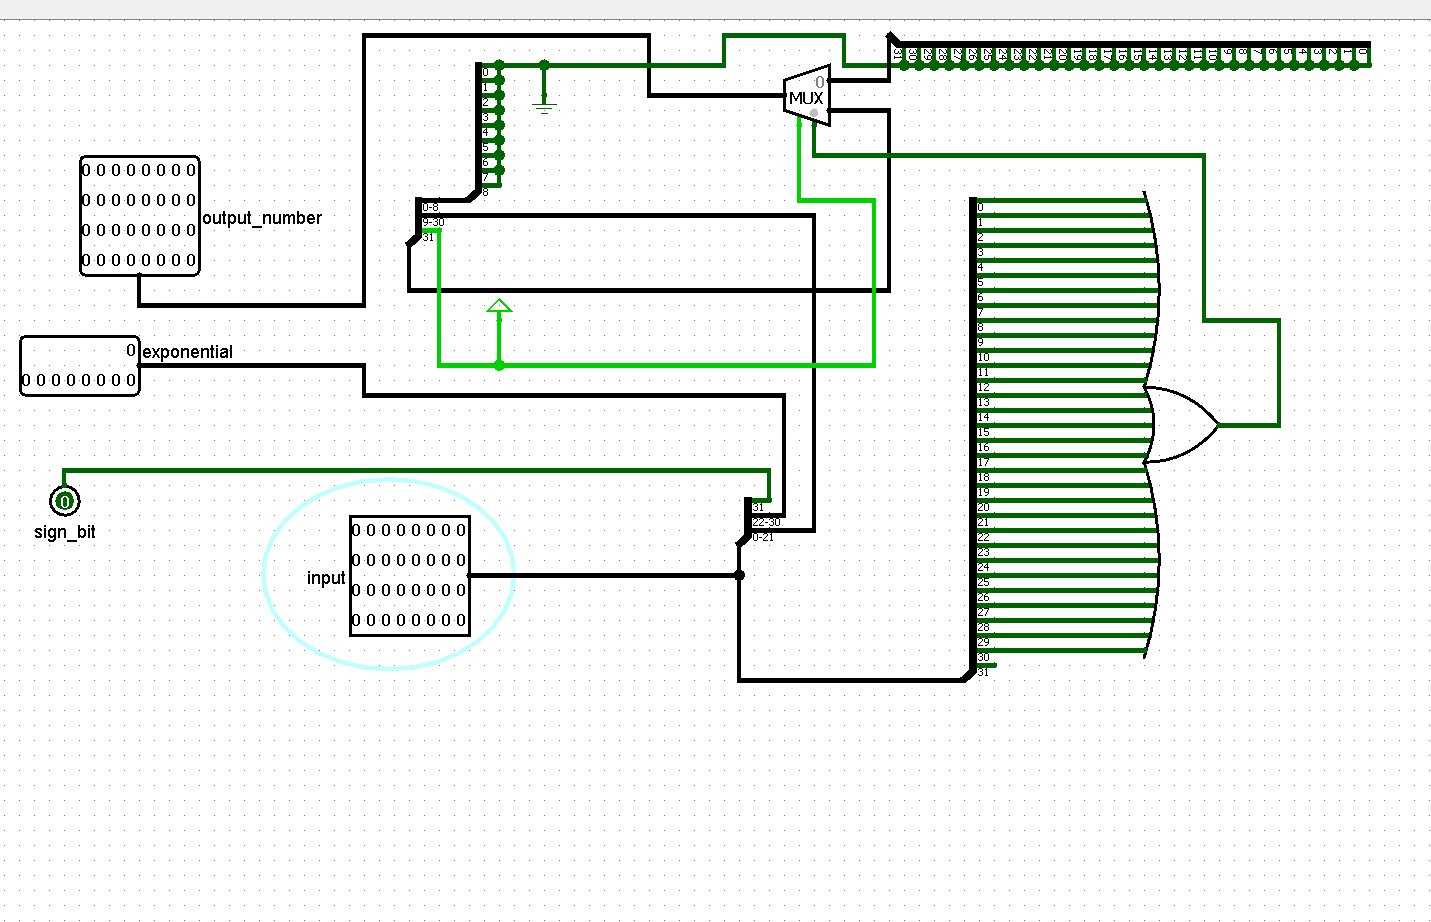
\includegraphics[width=0.4\textwidth]{mezba_image/input_process.png}}
    \hspace{1cm}
    \subfloat[Exponent Differentiator]{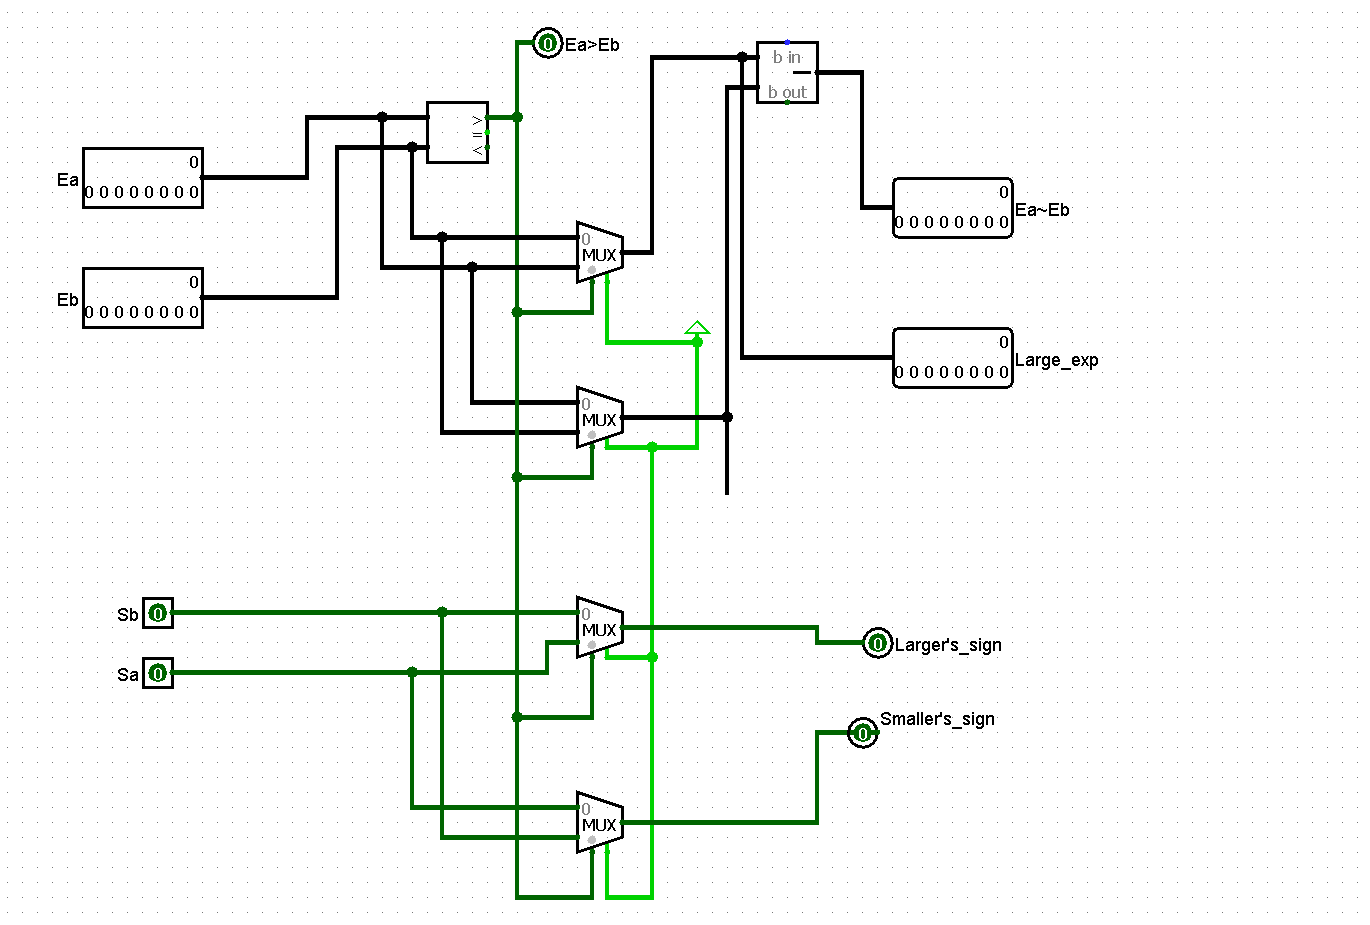
\includegraphics[width=0.4\textwidth]{mezba_image/Exp_process.png}}

    \hspace{1cm}
    \subfloat[Signifacant comparator]{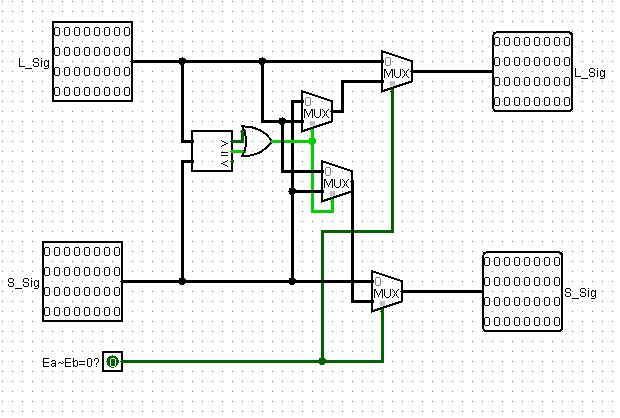
\includegraphics[width=0.4\textwidth]{sign_chooser.png}}
    \hspace{1cm}
    \subfloat[Sign comparator]{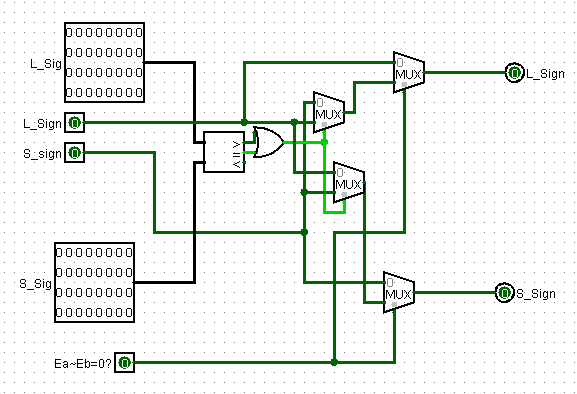
\includegraphics[width=0.4\textwidth]{sign_chose.png}}
    \hspace{1cm}
    \subfloat[Input Handler]{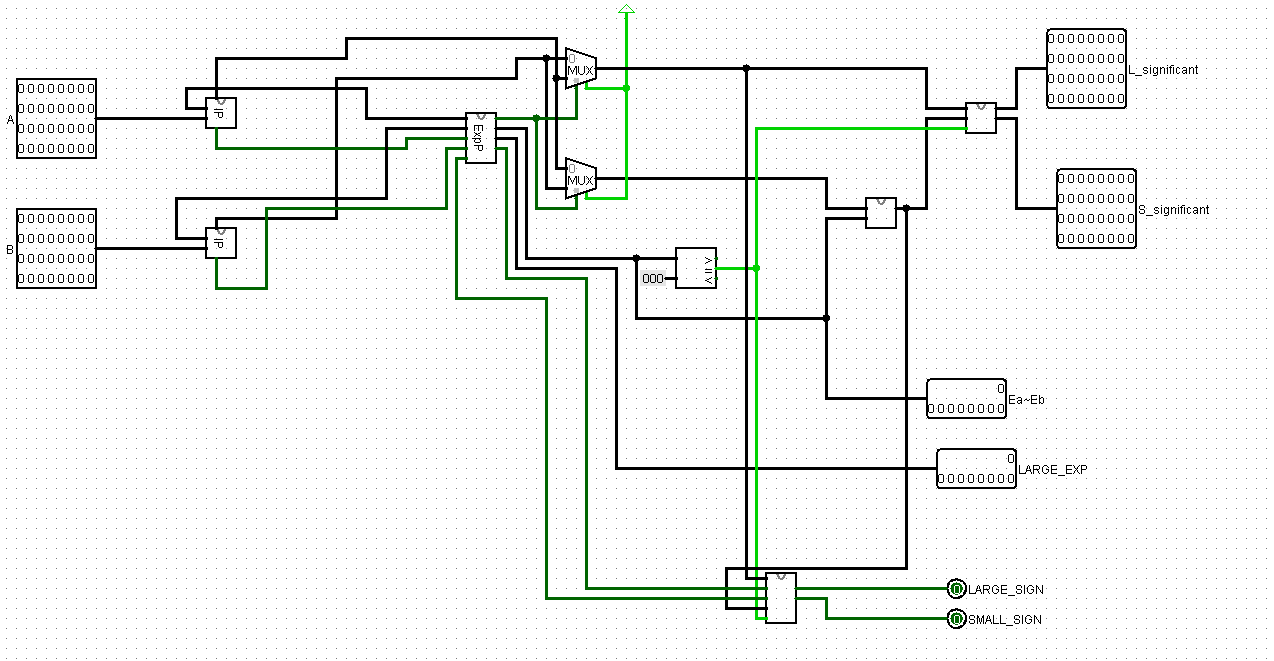
\includegraphics[width=0.5\textwidth]{input_processor.png}}

    \caption{Input Operator Modules}
    \label{fig:input_operator}
\end{figure}

\subsection{Adder Library}

The adder library contains circuits essential for performing floating-point
addition (FPA), including the following:

\begin{itemize}
    \item \textbf{32-Bit ALU:} A core component that performs addition or subtraction on the significands of two input floating-point numbers. It uses a control signal to toggle between addition (0) and subtraction (1) modes.

    \item \textbf{Significand Adder:} This unit manages the input significands, determining the operation type based on the signs of the inputs. Additionally, if the resulting significand is zero, it sets the output sign to zero.
\end{itemize}
\begin{figure}[H]
    \centering

    \subfloat[32-Bit ALU]{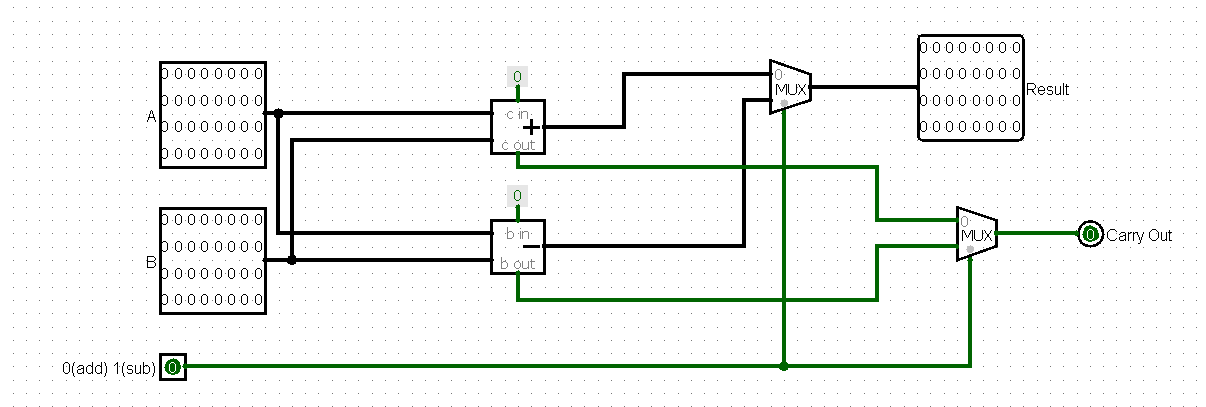
\includegraphics[width=\textwidth]{32bitalu.png}}
    \hspace{1cm}
    \subfloat[Significant Adder]{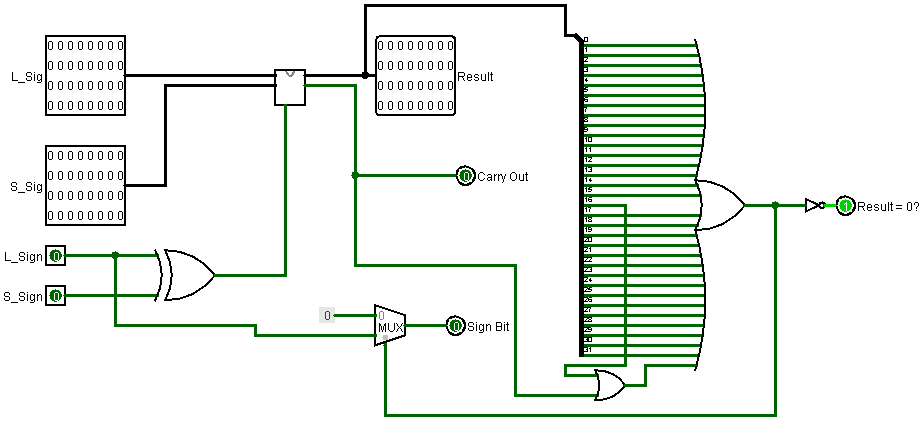
\includegraphics[width=.8\textwidth]{Significand Adder.png}}

    \caption{Adder Library}
    \label{Significand Adder}
\end{figure}

\subsection{Checker Library}
The 9 bit Zero Checker (\texttt{0\_checker.circ}) checks whether the Exponent's
all 9 bits are zero or not. Same for the 9 bit One Checker
(\texttt{1\_checker.circ}) whether the Exponent's all 9 bits are one or not.
The 32 bit Zero Checker (\texttt{32bit\_0\_checker.circ}) checks whether the
significand's all 32 bits are zero or not.

\begin{figure}[H]
    \centering
    % Row 1
    \begin{subfigure}[b]{0.45\textwidth}
        \centering
        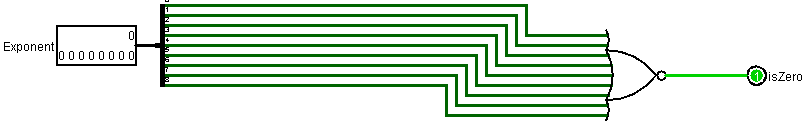
\includegraphics[width=\textwidth]{0_checker.png}
        \subcaption{9 bit Zero Checker}
    \end{subfigure}
    \hfill
    \begin{subfigure}[b]{0.45\textwidth}
        \centering
        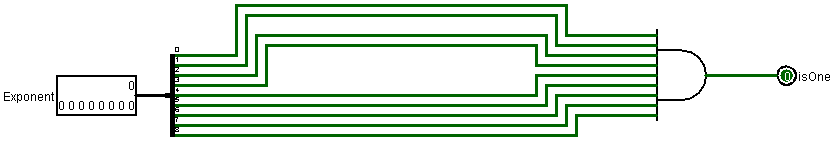
\includegraphics[width=\textwidth]{1_checker.png}
        \subcaption{9 bit One Checker}
    \end{subfigure}
    \hfill
    \begin{subfigure}[b]{0.45\textwidth}
        \centering
        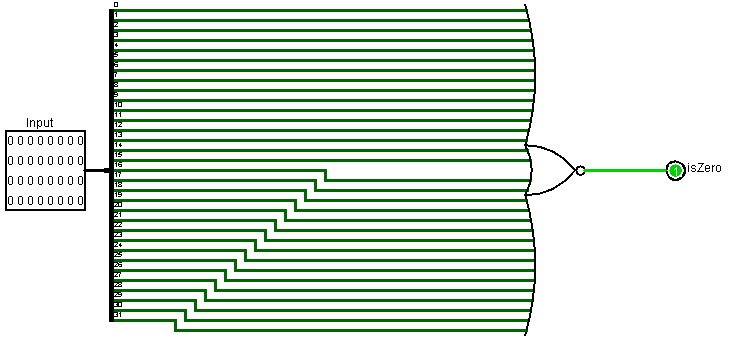
\includegraphics[width=\textwidth]{32bit_0_checker.png}
        \subcaption{32 bit Zero Checker}
    \end{subfigure}
    \caption{Checker Library}
\end{figure}

\subsection{Shifter Library}

\textbf{Left Shifters:Liberty} The left shifters can shift bits by 1, 2, 4, 8, or 16 positions:
\begin{itemize}
    \item \texttt{1 LeftShift} - Shifts left by 1 bit
    \item \texttt{2 LeftShift} - Shifts left by 2 bits
    \item \texttt{4 LeftShift} - Shifts left by 4 bits
    \item \texttt{8 LeftShift} - Shifts left by 8 bits
    \item \texttt{16 LeftShift} - Shifts left by 16 bits
\end{itemize}

\textbf{Right Shifters:} The right shifters can shift bits by 1, 2, 4, 8, or 16 positions:
\begin{itemize}
    \item \texttt{1 RightShift} - Shifts right by 1 bit
    \item \texttt{2 RightShift} - Shifts right by 2 bits
    \item \texttt{4 RightShift} - Shifts right by 4 bits
    \item \texttt{8 RightShift} - Shifts right by 8 bits
    \item \texttt{16 RightShift} - Shifts right by 16 bits
\end{itemize}

\textbf{Arbitrary Shifters:} These shifters can shift by any number of bits up to 31 bits:
\begin{itemize}
    \item \texttt{Arbitary LeftShift} - Shifts left by an arbitrary number of bits (up to 31)
    \item \texttt{Arbitary RightShift} - Shifts right by an arbitrary number of bits (up to 31)
\end{itemize}

\textbf{Right Shifter with Empty:} This shifter sets all bits to 0 if the shift amount exceeds 31 bits:
\begin{itemize}
    \item \texttt{Right Shift With Empty} - Right shifts up to 31 bits, or sets all bits to 0 if more than 31 bits
\end{itemize}

\begin{figure}[H]
    \centering
    % Row 1
    \begin{subfigure}[b]{0.3\textwidth}
        \centering
        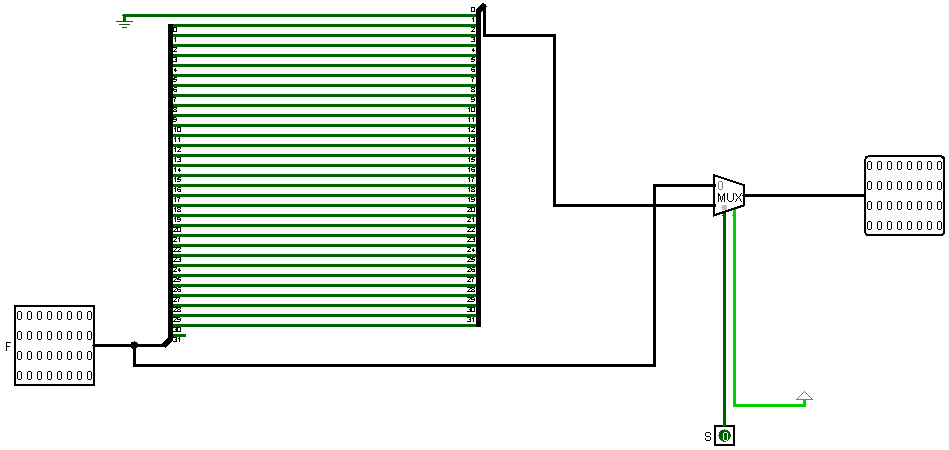
\includegraphics[width=\linewidth]{1 bit leftShifter.png}
        \subcaption{1 bit left shifter}
    \end{subfigure}
    \hfill
    \begin{subfigure}[b]{0.3\textwidth}
        \centering
        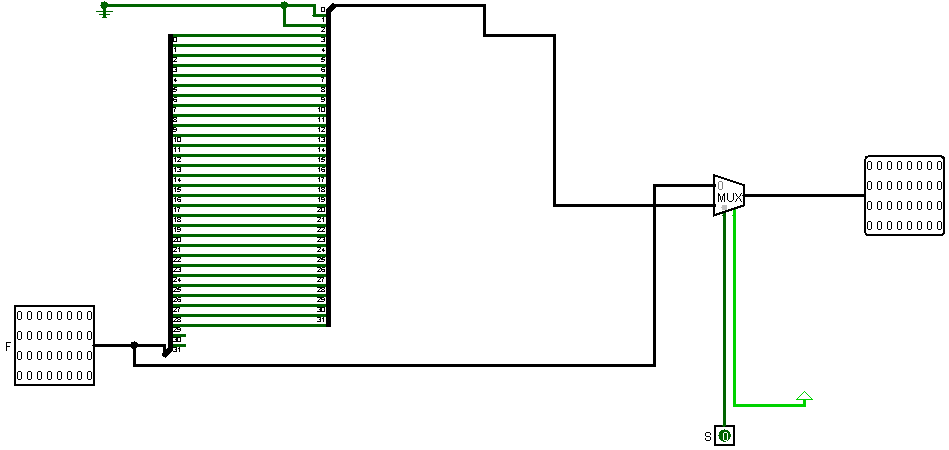
\includegraphics[width=\linewidth]{2 bit leftShifter.png}
        \subcaption{2 bit left shifter}
    \end{subfigure}
    \hfill
    \begin{subfigure}[b]{0.3\textwidth}
        \centering
        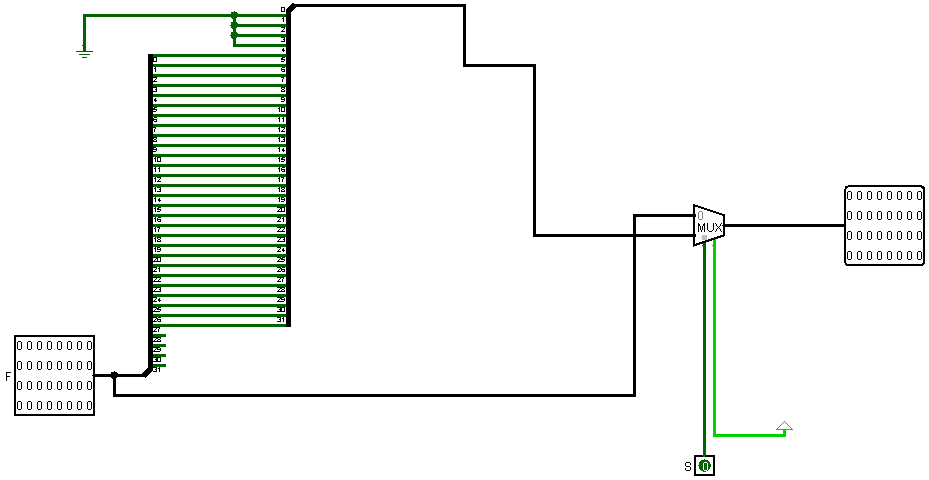
\includegraphics[width=\linewidth]{4 bit leftShifter.png}
        \subcaption{4 bit left shifter}
    \end{subfigure}
    \newline
    \newline
    \vspace{1em}

    % Row 2
    \begin{subfigure}[b]{0.3\textwidth}
        \centering
        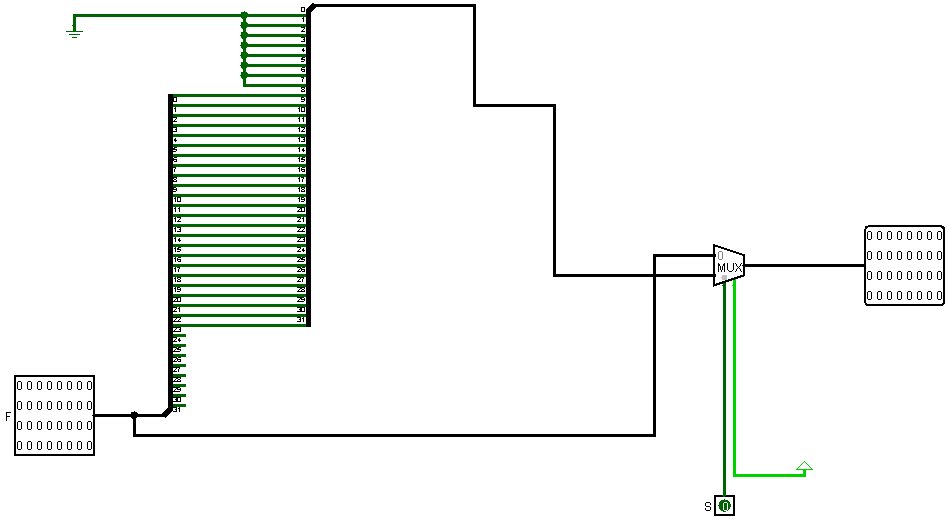
\includegraphics[width=\linewidth]{8 bit leftShifter.png}
        \subcaption{8 bit left shifter}
    \end{subfigure}
    \hfill
    \begin{subfigure}[b]{0.3\textwidth}
        \centering
        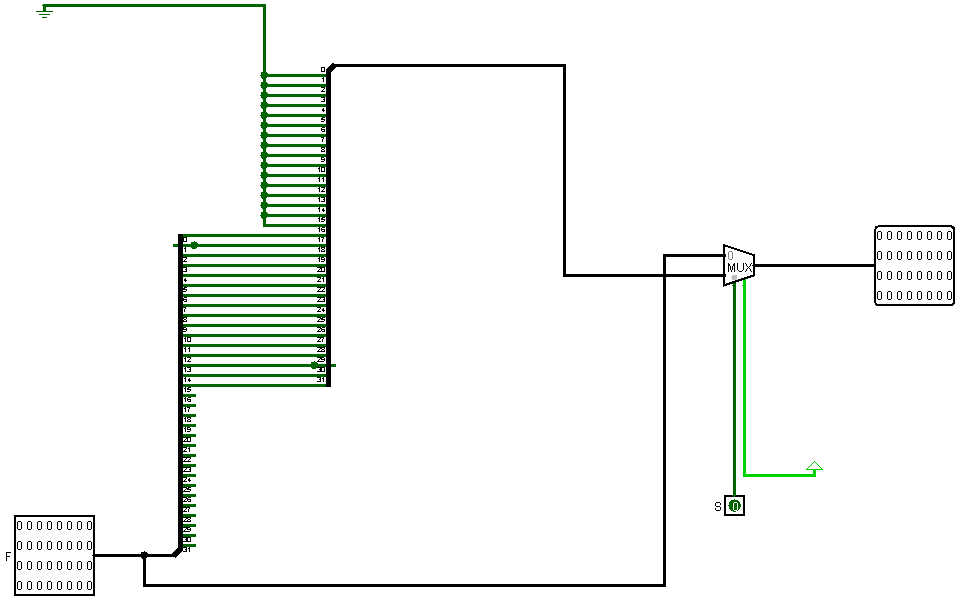
\includegraphics[width=\linewidth]{16 bit leftShifter.png}
        \subcaption{16 bit left shifter}
    \end{subfigure}
    \hfill
    \begin{subfigure}[b]{0.3\textwidth}
        \centering
        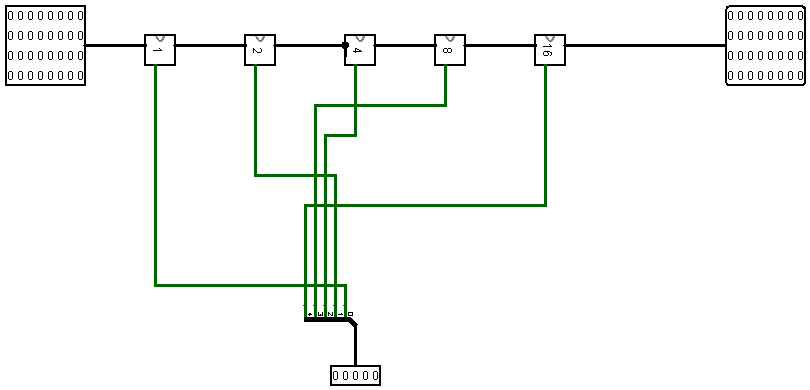
\includegraphics[width=\linewidth]{Arbitary leftShifter.png}
        \subcaption{Arbitary left shifter}
    \end{subfigure}
    \newline
    \newline
    \vspace{1em}

    % Row 3
    \begin{subfigure}[b]{0.3\textwidth}
        \centering
        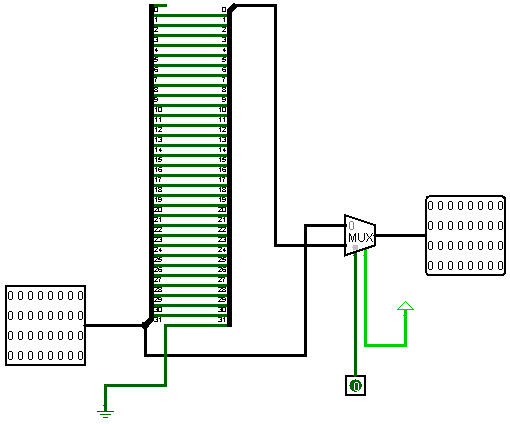
\includegraphics[width=\linewidth]{1 bit rightShifter.png}
        \subcaption{1 bit right shifter}
    \end{subfigure}
    \hfill
    \begin{subfigure}[b]{0.3\textwidth}
        \centering
        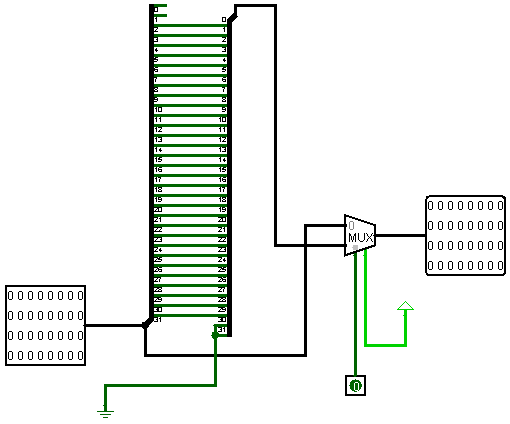
\includegraphics[width=\linewidth]{2 bit righShifter.png}
        \subcaption{2 bit right shifter}
    \end{subfigure}
    \hfill
    \begin{subfigure}[b]{0.3\textwidth}
        \centering
        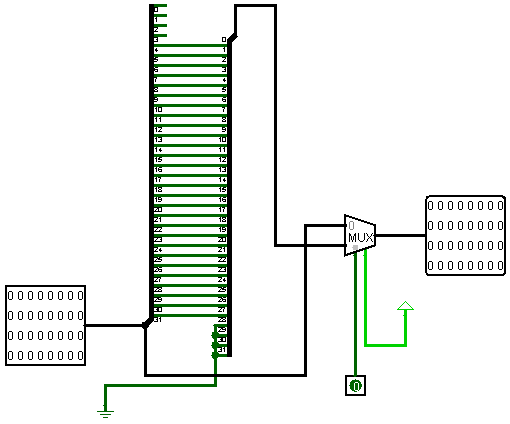
\includegraphics[width=\linewidth]{4 bit rightShifter.png}
        \subcaption{4 bit right shifter}
    \end{subfigure}
    \newline
    \newline
    \vspace{1em}

    % Row 4
    \begin{subfigure}[b]{0.3\textwidth}
        \centering
        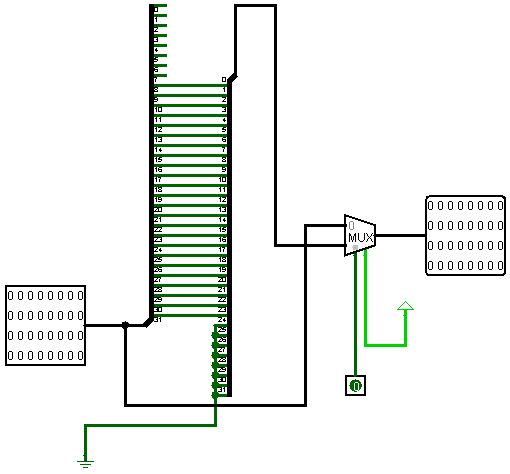
\includegraphics[width=\linewidth]{8 bit rightShifter.png}
        \subcaption{8 bit right shifter}
    \end{subfigure}
    \hfill
    \begin{subfigure}[b]{0.3\textwidth}
        \centering
        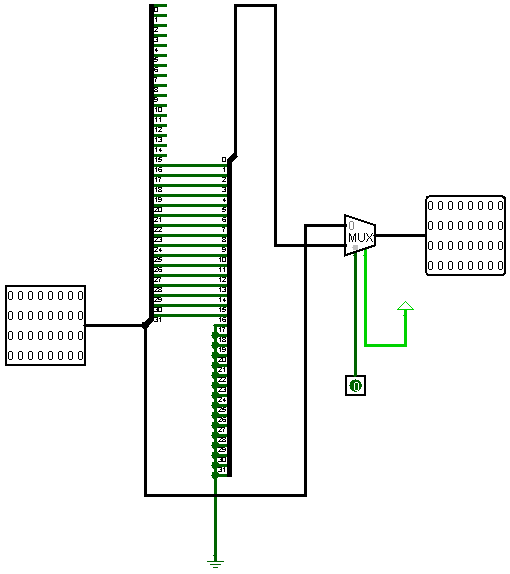
\includegraphics[width=\linewidth]{16 bit rightShifter.png}
        \subcaption{16 bit right shifter}
    \end{subfigure}
    \hfill
    \begin{subfigure}[b]{0.3\textwidth}
        \centering
        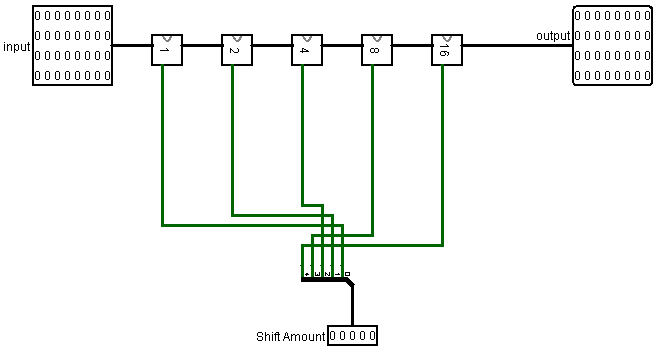
\includegraphics[width=\linewidth]{Arbitary RightShifter.png}
        \subcaption{Arbitary Right Shifter}
    \end{subfigure}
    \newline
    \newline
    \hfill
    \begin{subfigure}[b]{0.3\textwidth}
        \centering
        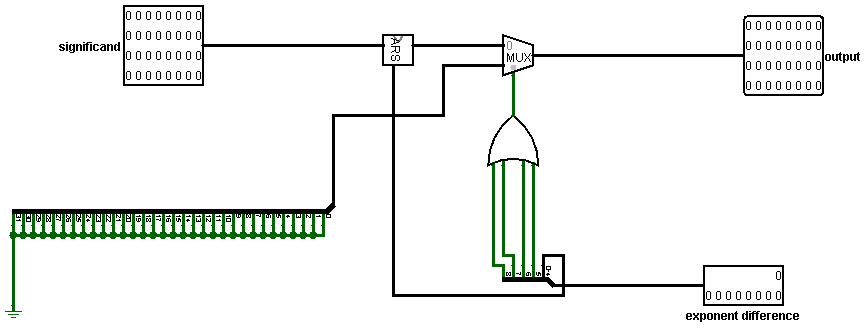
\includegraphics[width=\linewidth]{Right_Shifter.png}
        \subcaption{Right Shift with empty}
    \end{subfigure}
    \caption{Shifter Circuits}

\end{figure}

\pagebreak

\subsection{Normalizer Library}
This library contains 3 circuits. a 32 bit shifter, an 9 bit ALU(for addition
and subtraction) and a normalizer.
\begin{figure}[H]
    \centering
    \begin{subfigure}[h]{.4\textwidth}
        \centering
        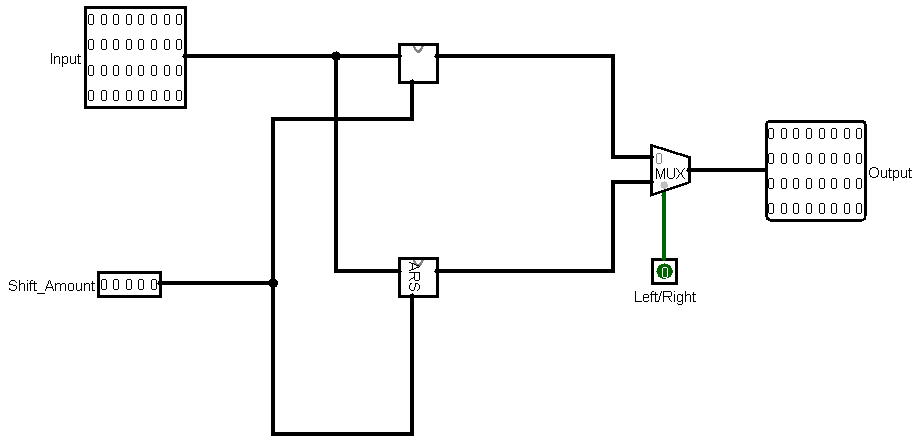
\includegraphics[width=1\textwidth]{normalizer_shifter.png}
        \caption{32 bit shifter}
    \end{subfigure}
    \hfill
    \begin{subfigure}[h]{.4\textwidth}
        \centering
        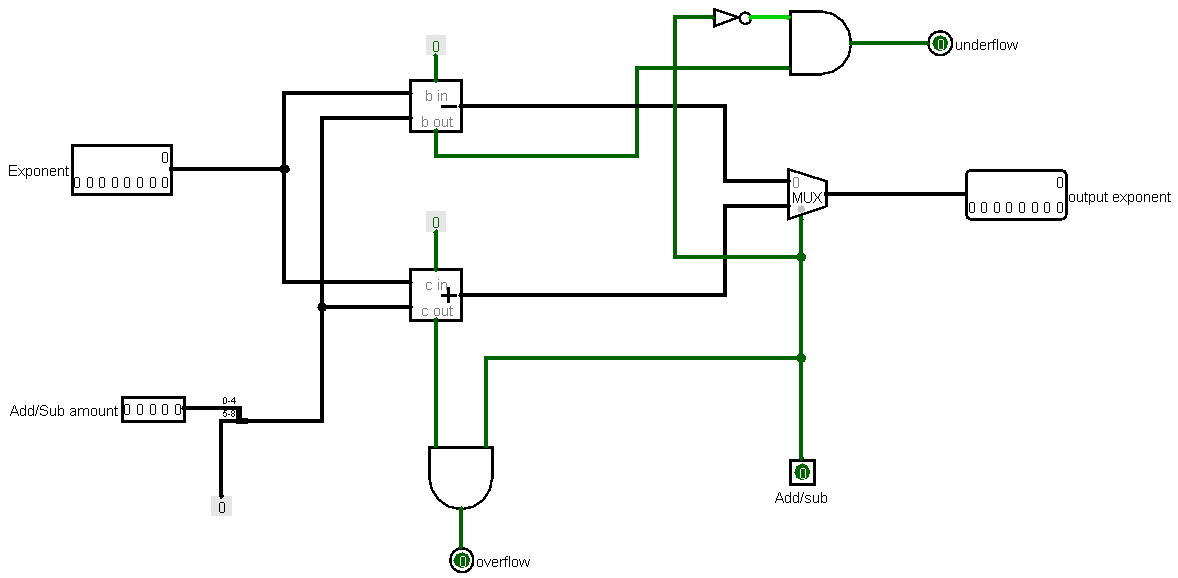
\includegraphics[width=1\textwidth]{norm_add_sub.png}
        \caption{9 bit ALU}
    \end{subfigure}
    \begin{subfigure}[h]{.8\textwidth}
        \centering
        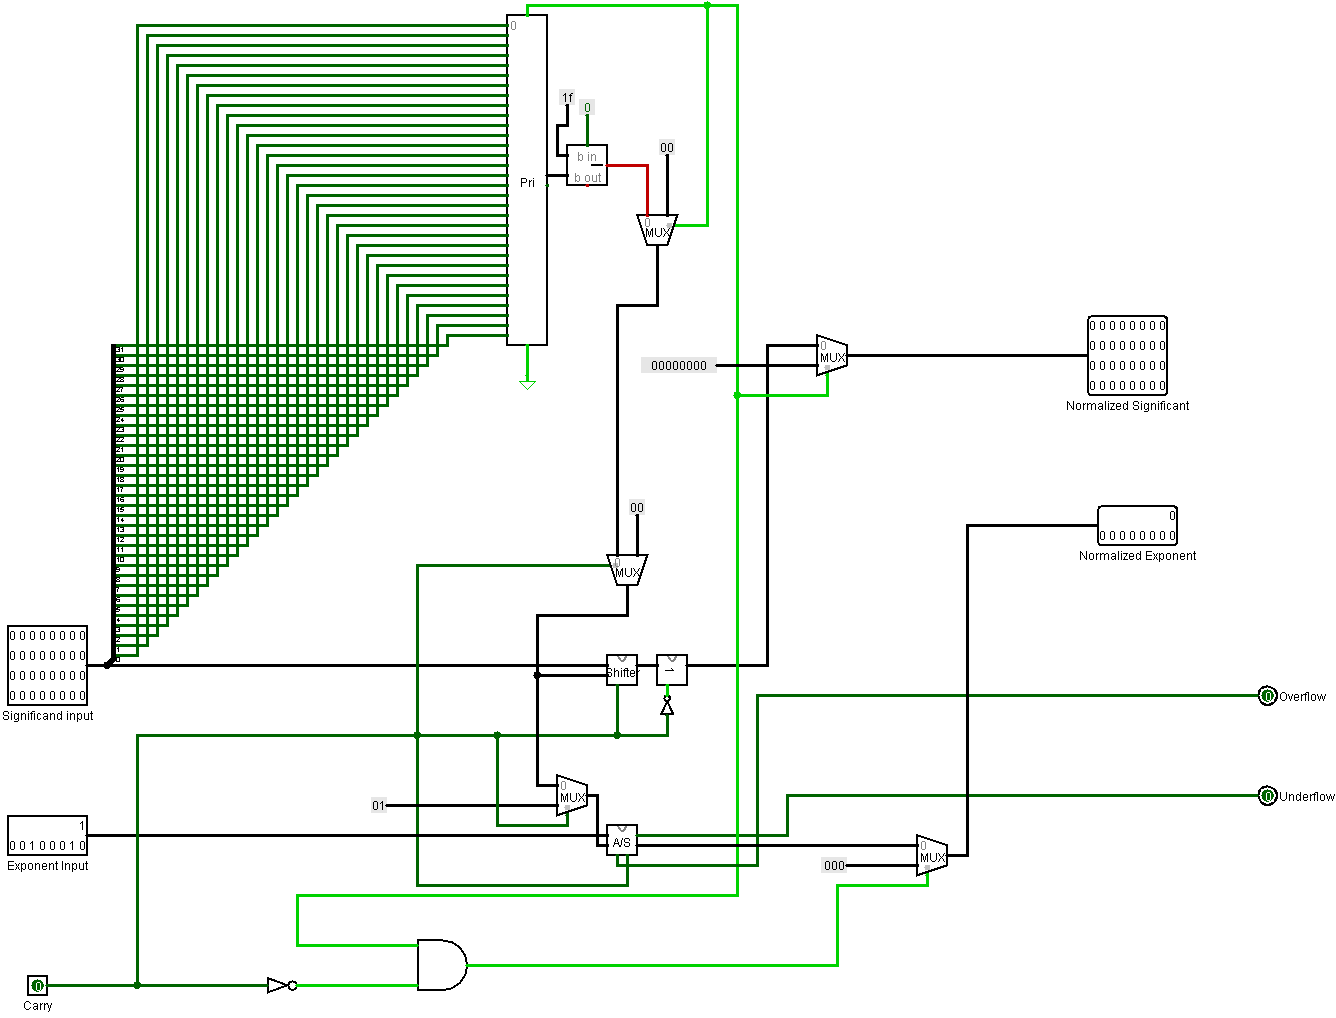
\includegraphics[width=1\textwidth]{normalizer.png}
        \caption{Normalizer}
    \end{subfigure}
    \caption{Normalizer Library}
\end{figure}

\subsection{Rounder}
The name of the Module is Rounder.circ. It contains two OR gate,one AND gate
and a full Adder and does the rounding of the mantissa.

\begin{figure}[H]
    \centering
    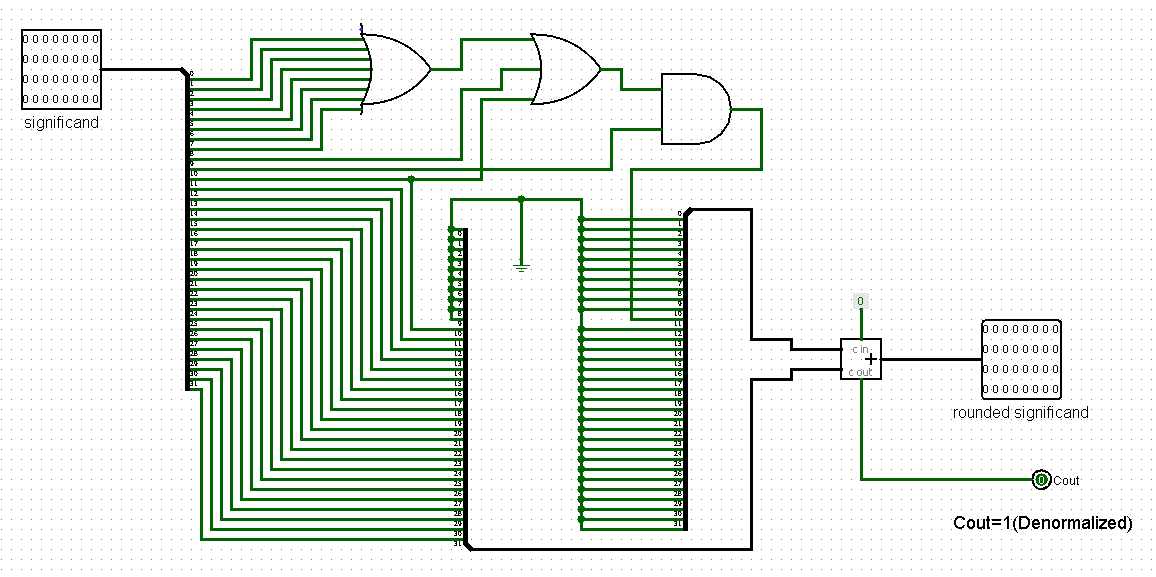
\includegraphics[width=1\textwidth]{R.png}
    \caption{Rounder Circuit}
    \label{rounder}
\end{figure}

\subsection{Rounded Normalizer}
Circuit to check whether the output from Rounder is normalized or not. If not,
it normalizes the result and also checks for overflow and normalization.

\begin{figure}[H]
    \centering
    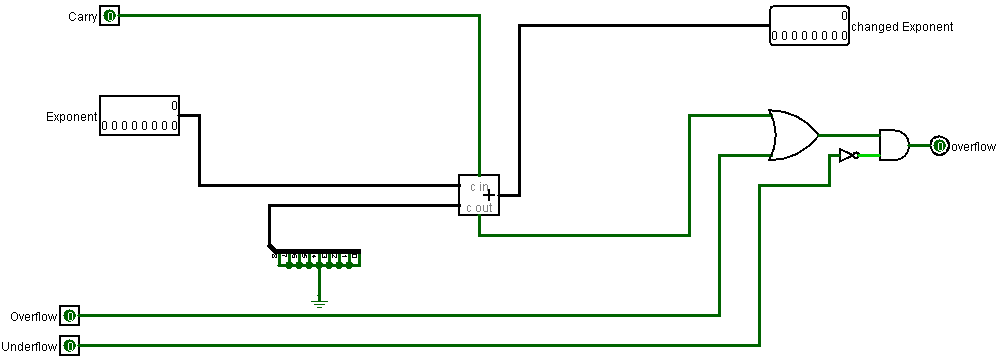
\includegraphics[width=1\textwidth]{RoundedNorm.png}
    \caption{Rounded Normalizer}
\end{figure}

\subsection{Flag Checker}
The flag checker[Flag.circ] checks the properties of the result whether the
result is denormalized or underflow or overflow or NaN or INF.

\begin{figure}[H]
    \centering
    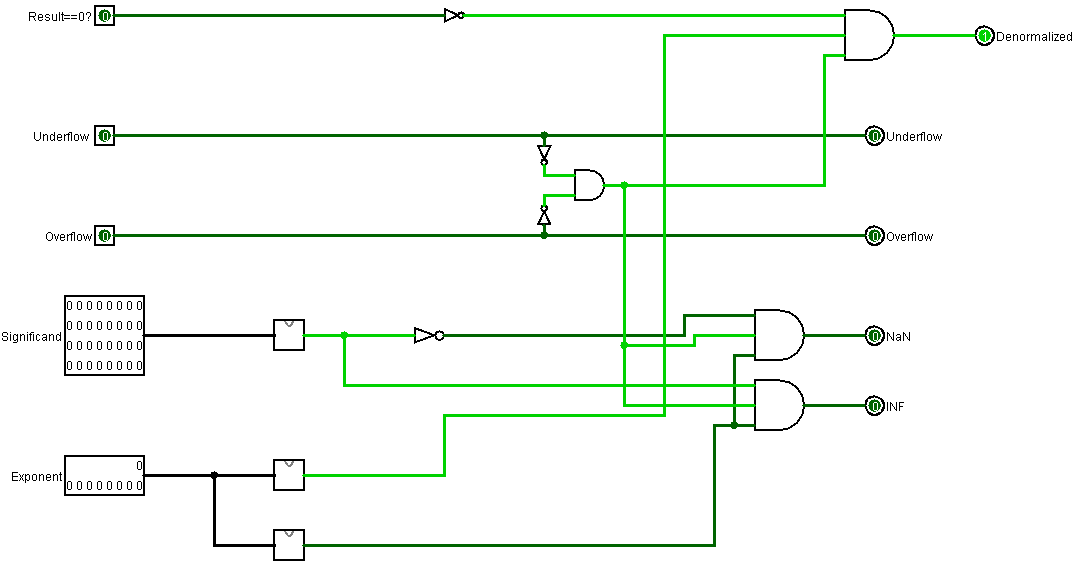
\includegraphics[width=1\textwidth]{Flag.png}
    \caption{Flag Checker}
    \label{Flag}
\end{figure}

\subsection{Output Presenter}
THis circuit is responsible for formatting the final output of a floating-point
computation. It takes as input a 1-bit sign, a 9-bit exponent, and a 32-bit
significand. The circuit combines these inputs by preserving the 1 sign bit, 9
exponent bits, and selecting the 22 most significant bits from the 32-bit
significand to create a standardized 32-bit output. This ensures the output
aligns with the desired floating-point format, effectively rounding the
significand to fit the 32-bit structure.
\begin{figure}[H]
    \centering
    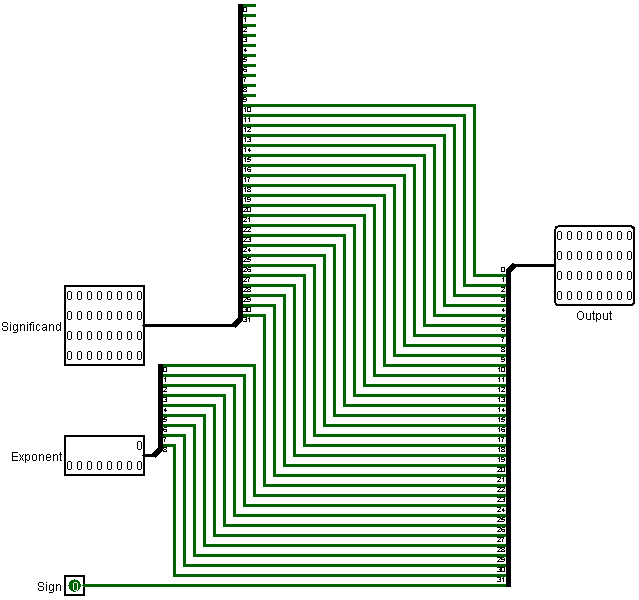
\includegraphics[width=1\textwidth]{Output.png}
    \caption{Output Processor of the Result}
    \label{Output}
\end{figure}

\section{Floating Point Adder}
The last module, called FPA.circ, uses the libraries and other modules to fully
create a floating point adder. It has the real floating point adder, or circuit
FPA. The output processor circuit that merges the sign, exponent, and
significand of the result is also included in this module.

\begin{figure}[H]
    \centering
    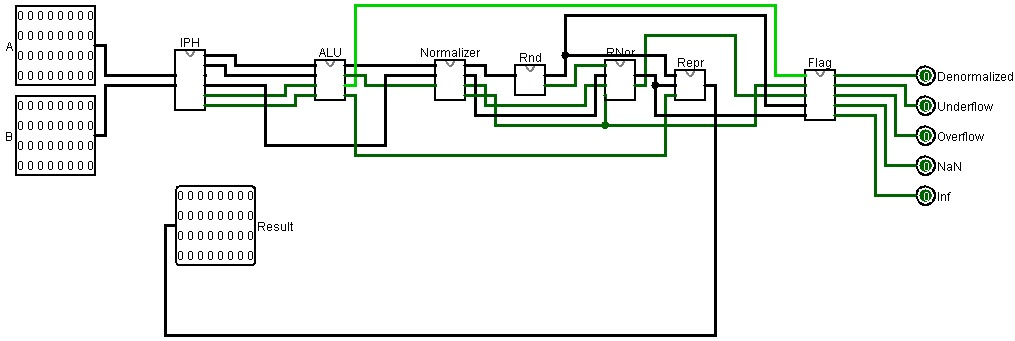
\includegraphics[width=1\textwidth]{FPA.jpg}
    \caption{The FPA}
    \label{FPA}
\end{figure}

\section{Flowchart of the Addition/Subtraction Algorithm}

\begin{figure}[H]
    \centering
    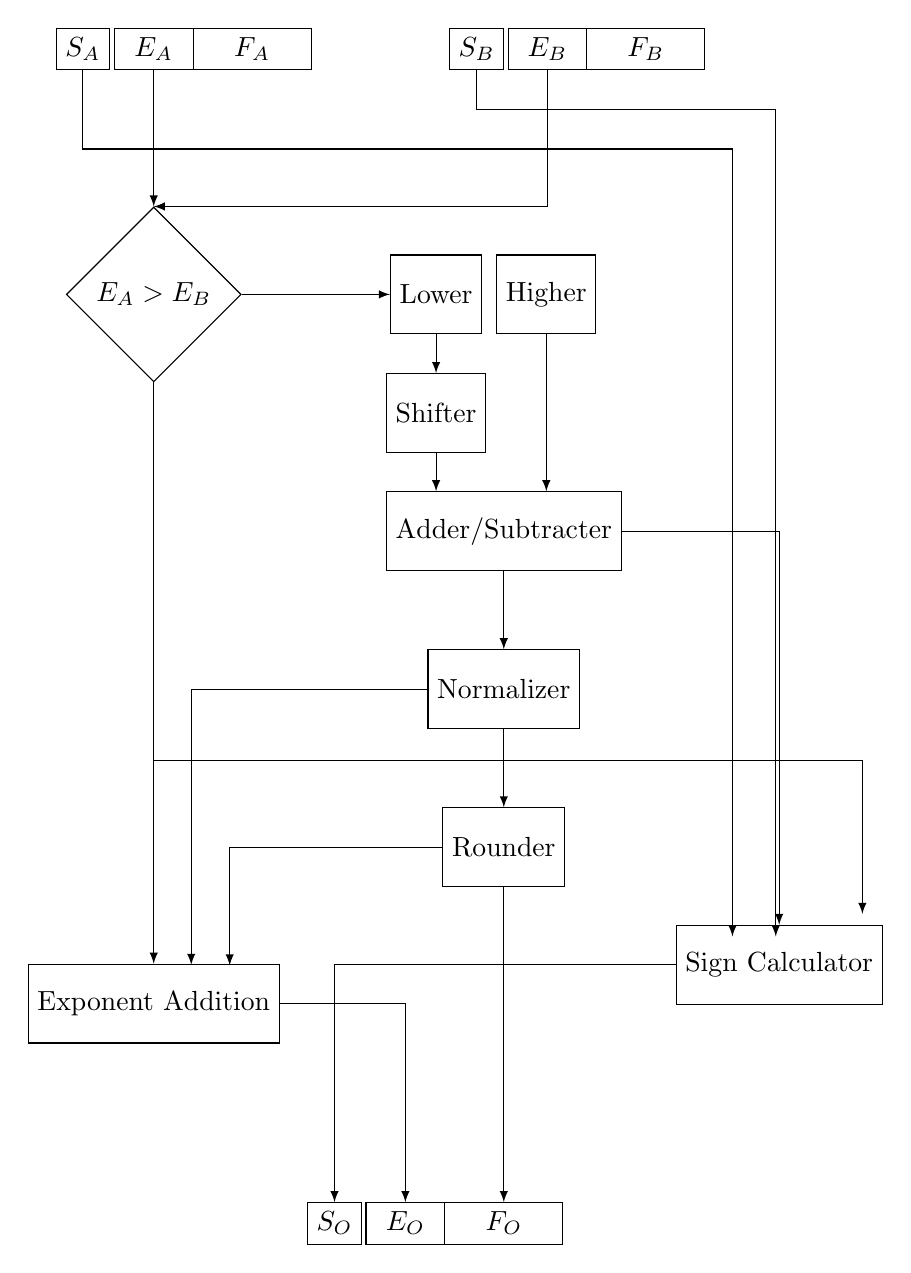
\begin{tikzpicture}
        \node[draw,
            minimum width=0.6cm,
            minimum height=0.5cm] (SA) at (0,0) {$S_A$};
        \node[draw,
            minimum width=1cm,
            minimum height=0.5cm] (EA) at ($(SA) + (.9, 0)$) {$E_A$};
        \node[draw,
            minimum width=1.5cm,
            minimum height=0.5cm] (FA) at ($(EA) + (1.25, 0)$) {$F_A$};

        \node[draw,
            minimum width=0.6cm,
            minimum height=0.5cm] (SB) at (5,0) {$S_B$};
        \node[draw,
            minimum width=1cm,
            minimum height=0.5cm] (EB) at ($(SB) + (.9, 0)$) {$E_B$};
        \node[draw,
            minimum width=1.5cm,
            minimum height=0.5cm] (FB) at ($(EB) + (1.25, 0)$) {$F_B$};

        \draw [-latex]
        (EA) --++(0, -2)
        node[diamond, draw, anchor=north] (comp) {$E_A>E_B$};

        \draw [-latex]
        (EB) -- (EB |- comp.north) -- (comp.north);

        \draw [-latex]
        (comp) --++(3, 0)
        node[draw,
            minimum width=1cm,
            minimum height=1cm, anchor=west] (low) {Lower};

        \node[draw,
            minimum width=1cm,
            minimum height=1cm] (high) at ($(low) + (1.4, 0)$) {Higher};

        \draw [-latex]
        (low) --++(0, -1)
        node[draw,
            minimum width=1cm,
            minimum height=1cm, anchor=north] (shift) {Shifter};

        \node[draw,
            minimum width=1cm,
            minimum height=1cm,
            anchor=west] (add) at ($(shift.west) + (0, -1.5)$) {Adder/Subtracter};

        \draw [-latex]
        (shift) -- (shift |- add.north);

        \draw [-latex]
        (high) -- (high |- add.north);

        \draw [-latex]
        (add) --++(0, -1.5)
        node[draw,
            minimum width=1cm,
            minimum height=1cm,
            anchor=north] (norm) {Normalizer};

        \draw [-latex]
        (norm) --++(0, -1.5)
        node[draw,
            minimum width=1cm,
            minimum height=1cm,
            anchor=north] (Rou) {Rounder};

        \draw [-latex]
        (comp) --++(0, -8.5)
        node[draw,
            minimum width=1cm,
            minimum height=1cm,
            anchor=north] (Eadd) {Exponent Addition};

        \draw [-latex]
        (Rou.west) --++(-2.7, 0) --++(0, -1.5);

        \draw [-latex]
        (norm.west) --++(-3, 0) --++(0, -3.5);

        \draw [-latex]
        (add.east) --++ (2, 0) --++(0, -5) node[draw,
            minimum width=1cm,
            minimum height=1cm, anchor=north] (sign) {Sign Calculator};

        \draw [-latex]
        (Rou.south) --++ (0, -4) node[draw,
            minimum width=1.5cm,
            minimum height=0.5cm, anchor=north] (FO) {$F_O$};

        \node[draw,
            minimum width=1cm,
            minimum height=0.5cm] (EO) at ($(FO) + (-1.25, 0)$) {$E_O$};

        \node[draw,
            minimum width=0.6cm,
            minimum height=0.5cm] (SO) at ($(EO) + (-0.9, 0)$) {$S_O$};

        \draw [-latex]
        (Eadd.east) -- (EO.north |- Eadd.east) -- (EO.north);

        \draw [-latex]
        (SA.south) --++ (0, -1) --++ (8.25, 0) --++ (0, -10);

        \draw [-latex]
        (SB.south) --++ (0, -0.5) --++ (3.8, 0) --++ (0, -10.5);

        \draw [-latex]
        (comp.south) --++ (0, -4.8) --++ (9.0, 0) --++ (0, -1.95);

        \draw [-latex]
        (sign.west) -- (SO.north |- sign.west) -- (SO.north);

    \end{tikzpicture}
    \caption{Flow chart of the addition/substraction algorithm}
\end{figure}

\section{\large{Comprehensive Design Description}}
\subsection{Comparing the Exponents and Aligning Radix Point}
The radix points need to be lined up in order to add two floating-point values.
To align the input with the larger input, this is usually accomplished by
moving the input with the smaller exponent to the right. We have computed the
difference between the two inputs using a 9-bit subtractor and compared their
exponents using a comparator.

\subsection{Shifting}
All shifting operations have been carried out using shifters based on
multiplexers. We have employed five 32-bit multiplexers to obtain bit shifts of
any arbitrary value up to 31. The multiplexers have the ability to shift 1, 2,
4, 8, and 16 bits in turn. Combining them yields shifts of any length up to 31,
as 3f and 3l illustrate. It could take more than 31 shifts to align two
fractions, in which case all bits would be 0. Furthermore, the exponent
difference ought to be the shifter circuit's input. Thus, after all seven of
the higher bits are clear, the lower five bits are used for shifting. The shift
amount does not exceed 31($2^{5}-1$) just in that scenario. Otherwise, the
fraction will be 0(all bits cleared), which is done in 3m.

\subsection{Normalization}
First we find out the location of first set bit using priority encoder. Then
subtract the location from from 32 to get the shift amount. We shift the
significand by the shift amount to the left and also decrease the exponent by
the shift amount. If we have carry from adder, we simply increase the exponent
by 1 and shift the significand by 1 to the left.

\subsection{Rounding}
We used a 32-bit adder to add and subtract the mantissas. However, we
occasionally need to round the result because we can only hold 22 bits. The
23st bit is regarded as the \textit{guard bit}, and the 24nd as the
\textit{round bit}. The \textit{sticky bit} will be set if any of the bits to
the right of the round bit are set; otherwise, it remains unset.
\begin{table}[h!]
    \centering
    \begin{tabular}{|c|c|c|c|c|}
        \hline
        22nd bit & G & R        & S        & Action   \\ \hline
        $\times$ & 0 & $\times$ & $\times$ & Truncate \\ \hline
        1        & 1 & $\times$ & $\times$ & Round up \\ \hline
        0        & 1 & 0        & 0        & Truncate \\ \hline
        $\times$ & 1 & 1        & $\times$ & Round up \\ \hline
        $\times$ & 1 & $\times$ & 1        & Round up \\ \hline
    \end{tabular}
\end{table}

Actually, \(X100\) is the case for round-to-even. So, if the 22th bit is 0, we
need to do nothing, hence truncation. Otherwise, we will round up. For
simplification, we will use a K-map. (22th bit = \(M\))

\begin{center}
\begin{karnaugh-map}[4][4][1][$RS$][$MG$]
\minterms{6,7,5,12,13,14,15}
\autoterms[0]
\implicant{5}{15}
\implicant{7}{14}
\implicant{12}{14}
\end{karnaugh-map}

\[
    \text{flag} = GS + GR + MG = G(M + R + S)
\]

\end{center}

If the flag is set, 1 is added at the 22th position. Otherwise, the bits beyond
the 23st position are truncated.

\subsection{Rounded Normalization}
This circuit adjusts the exponent of a floating-point number when a carry is
generated from the rounding process. If the rounding operation results in a
carry, this circuit increments the exponent by 1. Additionally, it includes
overflow detection to ensure that the incremented exponent does not exceed its
maximum value. If an overflow condition is detected, the circuit outputs a
signal to indicate the overflow, ensuring accurate handling of the
floating-point result within the specified range.

\subsection{Flag Checking}
The Flag Checking process is responsible for determining the status of the
floating-point result based on various conditions. It evaluates specific flags
such as Underflow, Overflow, Significand, and Exponent, to identify special
cases in floating-point arithmetic. Depending on these inputs, it assigns a
flag indicating one of several possible outcomes: $Denormalized, INF
    (\text{Infinity}), NaN (\text{Not a Number}), Underflow \text{ or } Overflow$.
This mechanism ensures proper categorization of edge cases, providing clarity
in scenarios where the result deviates from a normalized floating-point value.

\begin{table}[H]
    \centering
    \begin{tabular}{|ccccc|c|}
        \hline
        \multicolumn{5}{|c|}{Input}     & \multirow{2}{*}{Flag}                                                                                                                                                 \\ \cline{1-5}
        \multicolumn{1}{|l|}{Result=0?} & \multicolumn{1}{l|}{Underflow} & \multicolumn{1}{l|}{Overflow} & \multicolumn{1}{l|}{Significand} & \multicolumn{1}{l|}{Exponent} &                                   \\ \hline
        \multicolumn{1}{|c|}{0}         & \multicolumn{1}{c|}{0}         & \multicolumn{1}{c|}{0}        & \multicolumn{1}{c|}{0}           & 0                             & \multicolumn{1}{l|}{Denormalized} \\ \hline
        \multicolumn{1}{|c|}{$\times$}  & \multicolumn{1}{c|}{0}         & \multicolumn{1}{c|}{0}        & \multicolumn{1}{c|}{Not Zero}    & 0                             & \multicolumn{1}{l|}{Demornalized} \\ \hline
        \multicolumn{1}{|c|}{$\times$}  & \multicolumn{1}{c|}{0}         & \multicolumn{1}{c|}{0}        & \multicolumn{1}{c|}{0}           & 511                           & INF                               \\ \hline
        \multicolumn{1}{|c|}{$\times$}  & \multicolumn{1}{c|}{0}         & \multicolumn{1}{c|}{0}        & \multicolumn{1}{c|}{Not Zero}    & 511                           & NaN                               \\ \hline
        \multicolumn{1}{|c|}{$\times$}  & \multicolumn{1}{c|}{1}         & \multicolumn{1}{c|}{$\times$} & \multicolumn{1}{c|}{$\times$}    & $\times$                      & Underflow                         \\ \hline
        \multicolumn{1}{|c|}{$\times$}  & \multicolumn{1}{c|}{$\times$}  & \multicolumn{1}{c|}{1}        & \multicolumn{1}{c|}{$\times$}    & $\times$                      & Overflow                          \\ \hline
    \end{tabular}
    \caption{Flag Checking}
\end{table}

\section{ICs Used with Count as a Chart}

\begin{table}[H]
    \begin{center}

        \begin{tabular}{ll}
            \hline
            IC Number  & Quantity \\ \hline \hline
            IC 74157   & 183      \\ \hline
            IC 7432    & 43       \\ \hline
            IC 7408    & 15       \\ \hline
            IC 7483    & 72       \\ \hline
            Comparator & 4        \\ \hline
            IC 7402    & 3        \\ \hline
            IC 7404    & 4        \\ \hline
            IC 74148   & 4        \\ \hline
        \end{tabular}
    \end{center}
    \caption{IC count}
\end{table}

`
\section{Simulator used Along with the Version Number}
$logisim-generic-2.7.1$ has been used for simulating the floating point adder circuit.

\section{Discussion}
In our project, we aimed to implement a novel design of a Floating Point Adder
(FPA). Rather than designing the entire circuit from scratch, we opted for a
modular approach, building separate components first and then integrating them
to create a functional circuit. This strategy not only simplified the process
but also allowed us to distribute the workload effectively.\\

We encountered several challenges along the way. The first significant
challenge was designing a shifter capable of shifting by any arbitrary amount.
To achieve this, we combined 1, 2, 4, 8, and 16-bit shifters in a serial
configuration, where each shifter corresponded to one of the bits in the shift
amount.\\

The next challenge we faced to detect underflow and overflow. We checked for
underflow and overflow in our normalizer part. But for accurate output we again
had to check for overflow in our rounded normalizer part.\\

The toughest part of FPA was normalizer. Designing and testing the normalizer
took most of our time. But at last we made it and it works fine.\\

To ensure a minimal yet fully functional design, we used a combination of
built-in circuits from the Logisim library and our own custom circuits.\\

Overall, designing and implementing the floating-point adder was a rewarding
experience that deepened our understanding of its inner workings.

\section{Contribution}
\subsection*{2105151~~Md.Sani Alam Khan Piyes}
Rounder Circuit, Report Writing

\subsection*{2105152~~Sudip Kumar Saha}
Normalizer Library, Shifter Library, Checker Library, Testing, Report Writing

\subsection*{2105167~~Samyo Pramanik}
Initial Planning, Significand Adder Library, Normalizer, Flag Checker, Output
Presenter, Final FPA, Testing, Report Writing

\subsection*{2105172~~Mezba-Us-Saleheen}
Input Processor Library, Rounded Normalizer, Report Writing
\end{document}

\item 2105151 -- Md.Sani Alam Khan Piyes
\item 2105152 -- Sudip Kumar Saha
\item 2105167 -- Samyo Pramanik
\item 2105172 -- Mezba-Us-Saleheen